\chapter{Introduction -- Urban Computing} 
\label{chapter1:introduction}



\section{Urban Computing}

Urbanization's rapid progress has led to many mega cites, where people's lives have been enriched with advanced technology. Meanwhile new issues, such as air pollution and traffic congestion, pose greater challenges to us. To address these challenges, \emph{urban computing}~\cite{zheng2014urban} emerges as a means to unlock the power of big data from modern cites, to tackle the challenges faced by modern cities,  and to build more intelligent cities.

Nowadays, sensing technologies and large-scale computing infrastructure have produced a variety of \emph{big data} in urban spaces. In Figure~\ref{fig:intro}, we present an example of various data available in the City of New York. The big data have three major properties. 
\begin{enumerate}
\item Data variety. Urban data are collected in different formats. For example, crime data could be collected at incident level with detailed time and location. Meanwhile, demographic data are often reported at block level or community level.
\item Data volume. The quantity of urban data could be huge. For example, there are about 450,000 taxi trips are made in New York City every day according to the 2013 taxi data. There are over 380,000 venues on Foursquare as of 2015 in New York City, where people can visit and write reviews online.
\item Data velocity. The speed of new data being generated is fast. On average, there are 621 millions of tweets are generated every data according to the data collected in 2013.
\end{enumerate}

\begin{figure}[h]
\centering
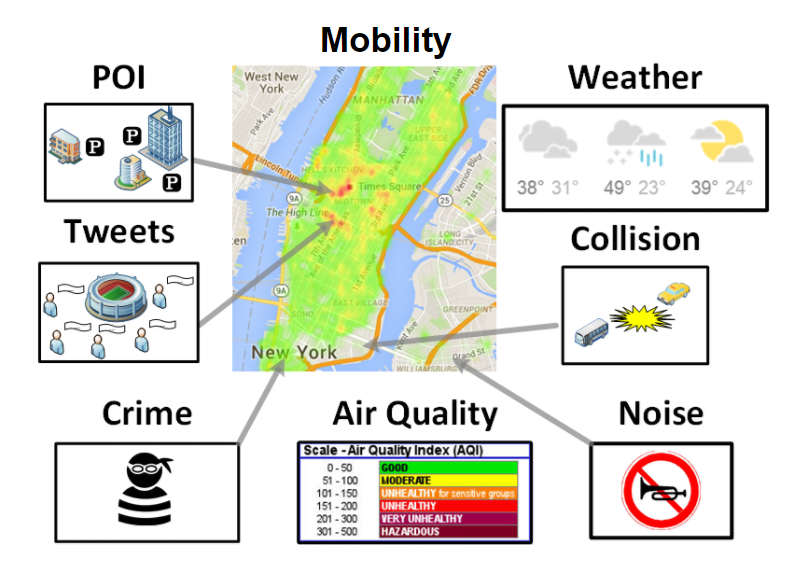
\includegraphics[width=0.8\linewidth]{fig/intro-data-v2.png}
\caption{Various big data collected in urban space.}
\label{fig:intro}
\end{figure}

All those urban data provide amazing opportunities for us to study urban problems and build intelligent urban applications. Among these data, the urban mobility data is especially interesting because the mobility flow connect a pair of locations. 


\section{Model Mobility-Flow-Incurred Interactions}


In the urban space, the movement of human population connects two disjoint regions, and brings influence from one to the other. My research focuses on modeling the complicated interactions in the urban space with human mobility data.  


In recent years, there are some large datasets of urban taxi made public~\cite{nyctaxi} under the Freedom of information request law.  The taxi dataset contains the time and location of pick-up and drop-off for a trip. By aggregating the taxi data, we are able to get the mobility flow among different regions.
Mobility flow data (e.g., commuting flow, taxi trajectories) are sensitive resources that urban planners can use to address city issues.




Consider the following two examples. These two examples show that it is not sufficient to only consider spatial interaction, and the interactions incurred by mobility flow is equally important.


\textbf{Example 1.} \emph{Policy makers are deciding where to construct a shelter for families that are victims of violence. They understand the value of locating the shelter geographically far from violent neighborhoods. One possible choice is to locate the shelter in a neighborhood that is 10 miles from the violent neighborhoods where vulnerable families previously lived. However, a deeper analysis may reveal that the new neighborhood, though geographically removed from the old neighborhood, may still have strong social flows (connections caused by commutes, family visits) with the old neighborhood. Emerging research suggests that a great deal of crime happens in areas that are socially connected to offenders' neighborhoods. This suggests that shelters may benefit from being located in a neighborhood that is also socially isolated from violence (e.g., with weak communication and commuting interactions with the violent neighborhoods that shelter residents fled from) while socially connected to jobs, services, and resources.}


\textbf{Example 2.} \emph{In order to provide better living environment to crowded city, city planner decide to expand city with a new satellite town. However, people are not willingly to move, if there is not enough incentive. To create opportunity and attract people, some candidates to relocate are big factory, shopping mall, and government offices. The question is which facility should be relocated, so that population pressure in whole  city  is relieved.  Correspondingly, how many new residential building, supermarket, and parks should be built into the new city? People have to go the new city to work. Some of them may move to live in the new city, and the rest may choose to commute everyday.}





\section{Research Problems}
\label{sec:qa}


In this dissertation, we model the city as a spatial network of regions, where each region is one node and there is a link between a pair of nodes. Links measure the interactions between a pair of regions. For example, the spatial link defines the spatial adjacency among regions. There are other types of links as well.  Accounting for these different types of region \textbf{interactions} can improve the a set of urban prediction tasks. I am specifically interested in the mobility flow data because they act as a type of ``hyperlink'' and connect regions that are spatially far away. In order to model the city as a spatial network, we have to answer the following three research questions.

\begin{itemize}
\item How to better understand nodes using links? In an urban prediction task, we usually estimate an unobserved property of a focal region from the observations of similar regions. The challenge lies in an appropriate definition of ``similar regions''. In the literature, spatial similarity is widely used. However, we argue that mobility flow also plays an important role in defining region similarity. For example, the crime rate in a residential neighborhood could be impacted by spatially non-adjacent but flow-connected neighborhoods.
\item How to define appropriate nodes in the spatial network? The administrative boundaries are widely used to define discrete regions. However, there are also a lot of concerns with the predefined boundaries. What if we do not have the boundaries available? What if the current boundary is outdated? Is the predefined boundary suitable for our prediction task?
\item What is the appropriate model for the correlations among various data in our spatial network? We argue that one global model cannot necessarily fit all scenarios. For example, nationwide we may observe that the house price is negatively correlated with house density. However, such observation is not universally true because we can easily find counterexample. For example, the house price in Manhattan island is high regardless of the high house density.
\end{itemize}




\section{Literature for Modeling Interactions of Networks}
\label{sec:ew}



\subsection{Spatial Interaction Model}


Spatial interaction is a broad term encompassing any movement over space that results from a human process \cite{haynes1984gravity,rodrigue2013geography}. It measures the flow between an origin and a destination, given distance and nodal properties on the origin and destination.  There are several classic models to measure the spatial interactions. For example, \textbf{gravity model} \cite{matyas1997proper} uses a similar formulation than Newton's law of gravity to model the interaction between two regions.
\textbf{Spatial autoregressive model} \cite{anselin1980estimation} is another widely used inference model that infer a property in a region with nearby region's information. There are a lot of  applications  based on the spatial interactions, such as international trade \cite{carrere2006revisiting, egger2003proper, martinez2003augmented}, population migration \cite{hanski1994metapopulation, karemera2000gravity, lewer2008gravity}, traffic flow \cite{jung2008gravity, roughan2002experience, khadaroo2008role}, telecommunication flow \cite{krings2009urban, fischer1994artificial, black1995spatial}, crime estimation \cite{anselin2000spatial, kakamu2008spatial, browning2004paradox}, knowledge spillover \cite{lesage2007knowledge, fischer2006geography}, and many more.



Notice that the region interaction in this thesis proposal is different from the traditional \textbf{spatial interaction} study, which assumes the interaction of two regions is reversely correlated with their geographical distance. However, space is a biased sample on human mobility, and should not be the only measure to model human movement. For example, during the weekdays people usually follow a regular home-office commuting pattern. The workplace region might be far from home region, but their connection is strong due to the human movement. As there are more and more mobility data available, we propose to employ the flow data in the interaction model as well.







\subsection{Exploring Mobility Flow}

In recent years, the availability of flow data enables research progress on exploring the role of various flows. New observations are made on the mobility data. For example, there are studies to explain epidemic spread with air travel \cite{huang2013global, tatem2014mapping} and population migration survey \cite{pindolia2013demographics}. Zheng et al. \cite{zheng2011urban} identify the underlying road network problem by detecting anomalous pair of flow. Yuan et al. \cite{yuan2012discovering} discover the function of regions by learning a topic model on the flow matrix and clustering the flow of region pairs into different topic.  Berlingerio et al. \cite{berlingerio2013allaboard} optimizes public transport route by looking at the region origin/destination flow. 



The problem in this proposal is different from the works above in the sense that different approaches are taken. Those works in the literature study the mobility flow by itself. Namely, the literature focuses on observing the properties of the mobility flow by various data mining technique, such as clustering \cite{berlingerio2013allaboard}, topic modeling \cite{yuan2012discovering}, outlier detection \cite{zheng2011urban} etc.  The approach in the literature uses the observed properties of flow to manually explain a phenomenon. This thesis proposal takes a different approach, that explicitly models the statistic dependency between social flow and region properties in an inference problem setting. The approach in this thesis allows us to answer those three research questions raised in Section~\ref{sec:qa}, which the literature methods cannot answer.





\subsection{Interaction Model in Social Networks}


In social network analysis, there is a line of work that focuses on infer an unobserved  nodal feature from neighboring nodes. Examples are infer user home location \cite{Pontes:2012:WKY:2370216.2370419, Li:2012:TSU:2339530.2339692}, user age \cite{6195711}, and more categorical features \cite{Mislove:2010:YYK:1718487.1718519}. Earlier works mainly focus on one type of features, and employ the network structure to make inference. To solve the application problem of user profiling, some techniques are borrowed from community detection \cite{fortunato2010community}, information diffusion \cite{guille2013information}, collaborative filtering \cite{breese1998empirical}, etc. The inferred features are assumed to be similar within a cluster. Therefore, community detection will cluster nodes with unobserved property together with nodes with observed property, and thus we can conduct inference. Another angle is to study how information is propagated through network. Methods under the information diffusion category is explanatory \cite{rodriguez2011uncovering, gomez2010inferring}.


With more data types available, there is one line of works solving the nodal feature inference problem with \textbf{composite social network} \cite{pan2011composite, madan2011pervasive,zhong2012comsoc}. Composite social network is a graph with multiple types of edges. For example in a social network, two users could be connected by following, how many re-tweets, how many messages are exchanged, etc. 


Our work is different from those work in social network literature in a way that we do not use observed edge strength as the interactions. All those paper in literature assumes that if two nodes are connected by a edge with heavy weight, then they are very likely to have strong interactions. This is not necessarily true. Take the crime inference as example. Suppose two communities are connected by heavy traffic flow, and both community are crime free. In this case, we cannot say two regions have strong crime interactions.







\section{Challenges}

There are mainly three challenges to address in modeling region networks through mobility flow.

\textbf{Given multiple types of social flow, the interaction is difficult to define}. Given only one type of social flow, there are too many possibilities in constructing interactions.  First, the flow matrix can take various form. For example, we can chose normalize the flow matrix or not. When normalizing the flow matrix, we can chose whether normalize by in-flow or out-flow. Second, there are many nodal properties that could interact with their neighbors, such as various demographics features. Third, different kinds of function can be used to define interactions. Take the product of flow and nodal properties is the most straightforward choice. However, sometimes it also makes sense to further apply distance exponential decay on previous product.  Furthermore, it is possible we have multiple types of social flow (e.g. taxi flow, commuter transit). For one pair of regions, should we build separate interaction over different social flows, or sum over all flows to get one interaction? When we take the sum, should we weight different social flow differently, and how?



\textbf{Constructing discrete node from continuous space is challenging}. In the literature, the boundary of regions are usually pre-defined administrative regions, which has two major issues. First, this boundary definition is not consistent in terms of the property of interest. For example, it is very likely a community is formed on the boundary of two administrative regions. Also, the current partition does not evolve over time. In real life, we know there must be some dynamic change of communities. Second, partition continuous space is not trivial. There is a misalignment problem, which refers to the problem that different data are not collected in the same scale. For example, the crime record is at point level, while the demographics is at block level.



\textbf{The interaction is non-stationary over the space}. Most models in existing work are global model, which assumes the statistic interaction does not vary over space. However, some urban data have spatial non-stationary property. Therefore, using global estimates of relationships can present misleading interpretations of local relationships.



\section{Organization}


The rest of my dissertation is organized as shown in Figure~\ref{fig:org}. In Chapter~\ref{ch:preliminary}, I give a preliminary study to verify the idea that using mobility flow as hyper-links to better model region similarity. We use crime inference as an example, in which we use an enhanced spatial autoregressive model to predict crime count of a community using its neighbors.

To address the aforementioned three challenges, I have correspondingly three chapters in my dissertation. We propose a graph embedding method to incorporate heterogeneous region interactions in Chapter~\ref{ch:embedding}. Next, we propose to automatically learn task-specific region partition in Chapter~\ref{ch:partition} to tackle the spatial continuity. In Chapter \ref{ch:non-stationary}, we first identify the spatial variations in mined relations. We further employ a geographically weighted regression model to solve the problem. Finally, I conclude in Chapter~\ref{ch:conclusion} with a discussion of potential future topics.


\begin{figure}[h]
\centering
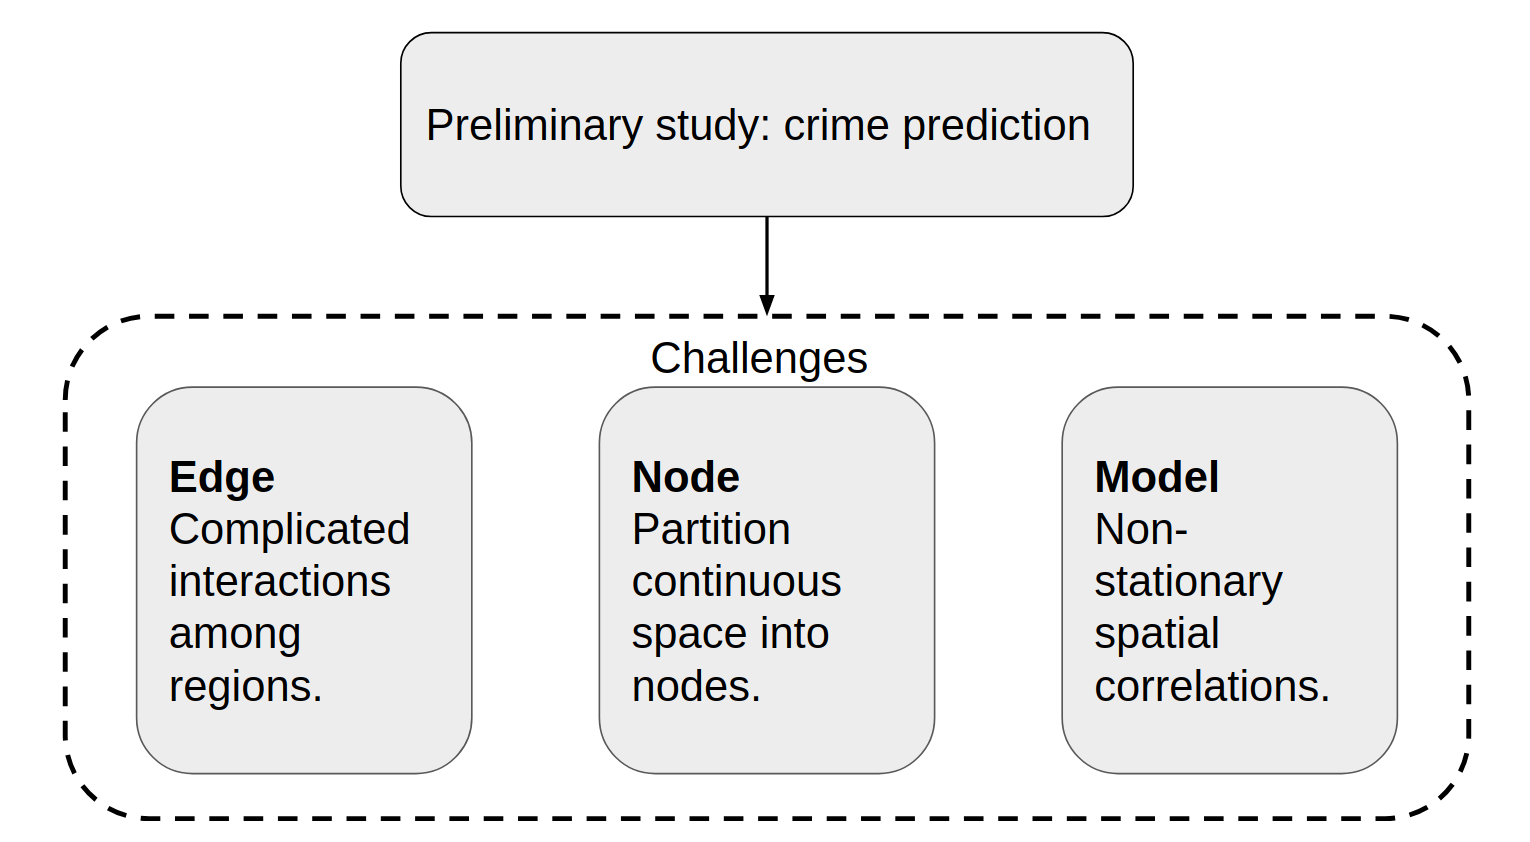
\includegraphics[width=\linewidth]{fig/organization.png}
\caption{Organization of this dissertation.}
\label{fig:org}
\end{figure}


